\section{\'Echantillonnage de signaux fondamentaux}

\begin{minipage}{0.4\linewidth}
  \refWeb{Corrigé \'Echantillonnage 1.1}{https://moodle.insa-toulouse.fr/mod/resource/view.php?id=104716}
\end{minipage}



\subsection{Premier ordre réel~: $e^{-t/\tau}$}

La réponse impulsionnelle d'un système continu du premier ordre est~:

$$ Y(p) = \frac{1}{1+\tau. p} X(p) \quad \underset{p.Y(p)\rightarrow \vec{\dot{y}} }{\longleftrightarrow} \quad \vec{y} + \tau \vec{\dot{y}}  = \vec{x}\quad \underset{\vec{x}=\vec{\delta_0}}{\longleftrightarrow} \quad \underbrace{h(t)}_{\vec{y}} =\frac{1}{\tau}. e^{-t/\tau}.\Gamma(t)$$


\def\h#1{(#1>0)}
\def\fonc#1{1 * \h{#1} *  exp(-#1)}
\def\dirac#1{(#1<0.001)*(#1>-0.001)*1}
%\begin{tikzpicture}
\begin{tikzpicture}[outer sep=auto, amp/.style = {regular polygon, regular polygon sides=3,
    draw, fill=white, text width=1em,
    inner sep=1mm, outer sep=0mm,
    shape border rotate=-90}]
  
  \matrix (graphe)[ row sep=0cm, column sep=1cm, inner sep=0.5cm]{ 	
  \begin{scope}[] 
    \begin{axis}[	anchor = origin,  x=1cm, y=1cm,
      axis lines=center, 
      xlabel={$t[s]$},
      ylabel={$\delta_0(t)$},
      ylabel style = {anchor=south, thick, black},
      xlabel style = {anchor=west, thick, black},
      grid=minor,
      domain=-0.5:2.5,
      ytick={0,1},
      yticklabels={0,1},
      xtick={0,1,2},
      xticklabels={0,1,2},
      enlarge y limits=0.5,
      enlarge x limits=0.1,
      help lines
      ]
      \addplot[very thick, blue,samples=512] plot (\x,{\dirac{\x}});
    \end{axis}
  \end{scope};
    & \node[dspnodeopen]  (x) {$\vec{x}$};
    & \node[dspsquare] (G) {$G(p)$} ;
    & \node[dspnodeopen]  (y) {$\vec{h}$};
    &
  \begin{scope}[] 
    \begin{axis}[anchor = origin,  x=1cm, y=1cm,
      axis lines=center, 
      xlabel={$t[s]$},
      ylabel={$h(t)$},
      ylabel style = {anchor=south, thick, black},
      xlabel style = {anchor=west, thick, black},
      grid=minor,
      domain=-0.5:3.5,
      ytick={0,1},
      yticklabels={0,$\frac{1}{\tau}$},
      xtick={0,1,2,3,4},
      xticklabels={0,$\tau$,$2\tau$,$3\tau$, },
      enlarge y limits=0.5,
      enlarge x limits=0.1,
      help lines
      ]
      \addplot[very thick, blue, samples=512] plot (\x,{\fonc{\x}});
      \draw[dashed, thick, blue](0,1)--(1,0);
    \end{axis}
  \end{scope}

    \\
  };
  \draw[dspflow] (x) -- (G) -- (y) ;
  
\end{tikzpicture}


Ce système de pôle $\widehat{p_c}=\frac{-1}{\tau}$ est stable
s.s.i. $\tau> 0$ car~:

Stable simple $\quad \iff h(t) \underset{t\to +\infty}{\rightarrow} 0 \iff$ \og{} retour à l'équilibre après stimuli. \fg{} 

Cela corrobore le fait qu'un pôle réel est stable s.s.i
$\widehat{p_c}$ est dans le demi-plan gauche de \Laplace{}~:
$\widehat{p_c}\prec 0$.

Le terme $\Gamma(t)$ est nul pour $t<0$ (fonction de \Heaviside), on
trouve que le système est causal puisque la Réponse ImPulsionnelle
(RIp) est nulle avant la stimulation par l'impulsion~:

Système causal $\quad \iff \quad \forall t<0,\; h(t)=0 \quad \iff$ \og{} pas de réponse avant stimuli. \fg 

\question{Q1~: discrétisation de $h$} Discrétisez le signal $t\mapsto h(t)$, avec
une période d'échantillonnage temporelle $T_e$, pour obtenir le signal
$\vec{h} : k \mapsto h[k]=h(\overbrace{k\,T_e}^{t})$.

Montrez qu'il s'agit d'une suite géométrique $h[k]=a^k.\Gamma[k]$ où
vous exprimerez $a\in\R$ en fonction de $\tau$ et $T_e$.

\question{Q2~: condition de stabilité en discret} Dans l'exercice AR~(Auto Regressif)~\ref{sec:AR}, nous construirons le système discret dont la réponse impulsionnelle est $k\to h[k]$ pour obtenir un système du premier ordre discret. 

Représentez $h$ graphiquement (discret et continu si possible) pour $a=\frac{1}{2}$, puis $a=1$, puis
$2$, puis $a=-\frac{1}{2}$, puis $-1$, puis $-2$.

La condition de stabilité simple en discret reste \og{}retour à zéro
après stimuli\fg{} :
  $h[k]\underset{k\to +\infty}{\longrightarrow} 0$.

  Donnez la condition nécessaire et suffisante de stabilité du système
  $H$ en fonction de $a$ et vérifiez qu'elle correspond à celle en
  continu avec $\tau$.
  
\subsection{Oscillateur imaginaire pur : $e^{i\omega\,t}$}
Le système du premier ordre précédant peut être choisi avec un pôle
imaginaire pur $p_c= i\omega$.

$$ Y(p) = \frac{1}{p-i\omega} X(p) \quad \underset{p.Y(p)\rightarrow \vec{\dot{y}} }{\longleftrightarrow} \quad  \vec{\dot{y}} - i\omega \vec{y}  = \vec{x}\quad \underset{\vec{x}=\vec{\delta_0}}{\longleftrightarrow} \quad \underbrace{h(t)}_{\vec{y}} = e^{i\omega\,t}.\Gamma(t)$$


Le système devient un système complexe (abstrait) de réponse
impulsionnelle $h(t)=e^{i\omega\,t}.\Gamma(t)$ comportant en partie
réelle une RIp (Réponse Impulsionnelle) $\cos\!\left(\omega\,t\right)$
causal et un $\sin\!\left(\omega\,t\right)$ causal en partie imaginaire.

\question{Q1~: discrétisation de $h$} Discrétisez le signal
$t\mapsto h(t)$, avec une période d'échantillonnage temporelle
$T_e$. Montrez qu'il s'agit, là aussi, d'une suite géométrique
$h[k]=q^k.\Gamma[k]$, mais cette fois-ci avec $q\in\C$ dont vous
donnerez la relation avec $\omega$ et $T_e$.

\question{Q2~: condition de stabilité en discret} Le pôle continu
$p_c$ correspond à un système en limite de stabilité, car la RIp $h$
ne converge pas vers 0 et ne diverge pas à l'infini non plus. Ce pôle est sur l'axe imaginaire pur~: entre le demi plan gauche stable et
le demi plan droit instable divergent.

Nous verrons plus tard que $q$ est le pôle du système discret.

Déterminez le type de convergence de $\left\{h[k]\right\}$. Que devient l'axe imaginaire de limite de stabilité pour les pôles continus $p_c$ lorsque l'on passe à un système discret de pôle $q$ ?

\question{Q3~: périodicité du spectre}

Pour représenter la suite numérique complexe $\left\{h[k]\right\}$
graphiquement, on placera les points $h[k]\in\C$ dans le plan
complexe en indiquant leur indice $k$ à côté.

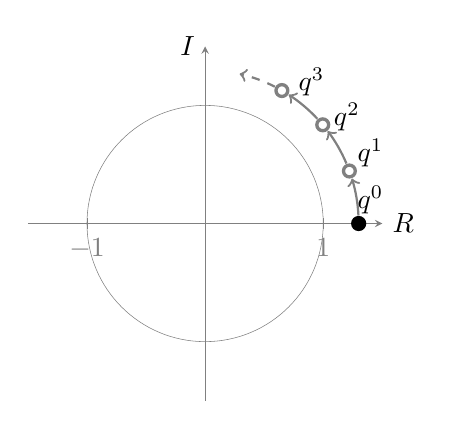
\begin{tikzpicture}

	\begin{axis}[
			anchor = origin,  x=1.5cm, y=1.5cm,
			ymin=-1.5, ymax=1.5,
			xmin=-1.5, xmax = 1.5,
			ytick = {0},	
			xtick={-1,1 },
			axis lines=center, 
			xlabel={$\mathbb{R}$},
			ylabel={$\mathbb{I}$},
			ylabel style = {anchor=east, thick, black},
			xlabel style = {anchor=west, thick, black},
			grid=minor,
			help lines]
 		\draw (0,0) circle (1);
		\draw [very thick, black, fill=black] ({1.3*cos(0)},{1.3*sin(0)}) circle (0.05) ;
		\draw [very thick] ({1.3*cos(20)},{1.3*sin(20)}) circle (0.05) node[right] {} ;
		\draw [very thick] ({1.3*cos(40)},{1.3*sin(40)}) circle (0.05) node[right] {} ;
		\draw [very thick] ({1.3*cos(60)},{1.3*sin(60)}) circle (0.05) node[right] {} ;
		\draw [thick,->] ({1.3*cos(3},{1.3*sin(3)}) arc (3:17:1.3)  node[right] {} ;
		\draw [thick,->] ({1.3*cos(23)},{1.3*sin(23)}) arc (23:37:1.3) node[right] {} ;
		\draw [thick,->] ({1.3*cos(43)},{1.3*sin(43)}) arc (43:57:1.3) node[right] {} ;
		\draw [thick,->,dashed] ({1.3*cos(63)},{1.3*sin(63)}) arc (63:77:1.3) node[right] {} ;
		\node [black ,  thick] (q0) at (1.4,0.2) {$q^0$};
		\node [black ,  thick] (q1) at (1.4,0.6) {$q^1$};
		\node [black ,  thick] (q2) at (1.2,0.9) {$q^2$};
		\node [black ,  thick] (q3) at (0.9,1.2) {$q^3$};
\end{axis}

\end{tikzpicture}

Représentez graphiquement $\vec{h}$ pour $q=e^{i\,\frac{\pi}{2}}$,
vous remarquerez que ce signal est $4$ périodique~: on le notera
$h_4$.

Représentez alors la suite numérique $h_4$ par un tuple de
4 valeurs complexes~:

$\ldp\overbrace{1}^{k=0},q, q^2, q^3\rdp = \ldp q^3, \overbrace{1}^{k=0},q, q^2 \rdp=\dots$ où les doubles parenthèses indiquent que la suite est périodique.

Faites de même avec $q=e^{i\,\frac{5\pi}{2}}$ et
$q=e^{i\,\frac{-3\pi}{2}}$. Cela devrait vous aider à trouver,
pour une pulsation d'échantillonnage
$\omega_e=2\pi\,F_e=\frac{2\pi}{T_e}$ donnée, \textbf{TOUTES}
les pulsations $\omega$ qui permetttent d'avoir ce signal
discret 4 périodique $h_4$.

\begin{remarque}
  On en déduit que toute les ondes continues pures de
  pulsation $\omega + n.\omega_e$, et donc de fréquence
  $f + n.F_e$, donnent exactement le même signal discret~!

  Lorsque l'on observe un signal fini de N échantillons, la
  transformée de \Fourier{} d'un Signal Discret (TFSD) étend ce signal
  par des zéros pour obtenir la suite infinie

  
  $( \dots,0,0, \overbrace{s[0]}^{}, \dots s[N-1],0,0,\dots)$ à
  support borné.

  
  Il suffit de décomposer/calculer la TFSD uniquement pour les
  fréquences $f \in \left[0 , F_e\right[$. En effet, la composante
  discrète à la fréquence $f$ est $e^{i\,2\pi\,f\,\frac{k}{F_e}}$ et
  un calcul pour une fréquence $f + n.F_e$ donnerait le même résultat
  que pour $f$ puisque on aurait exactement le même signal discret.

  Un signal discret est ainsi transformé par \textbf{la TFSD en
    fonction continue de $f$ qui est $F_e$ périodique} et seule les
  fréquences $0\le f<F_e$ sont utiles.
  
  Seul l'incrément angulaire $\Delta$ de
  $q=e^{i.\overbrace{2\pi\frac{f}{F_e}}^{\Delta}}$
  identifie une onde pure discrète. On
  préfère alors  utiliser la \textbf{fréquence normalisée}
  $\frac{f}{F_e}$, notée $\tilde{f}$.
  
\end{remarque}

\question{Q4 : signaux temporel  périodiques et spectre discrets}

On cherche maintenant toute les fréquences pouvant donner un signal
temporel de période 8.  Représentez graphiquement le signal de
fréquence normalisée $\tilde{f_0}=\frac{1}{8}$ pour
$q=e^{i\,2\pi\frac{1}{8}}$ et vérifiez la question précédente avec les
fréquences $\tilde{f}=\frac{9}{8}$ et $\tilde{f}=\frac{-7}{8}$ par
périodicité du spectre en fréquence.


Donnez la séquence $\ldp \overbrace{1}^{},\dots, q^7 \rdp$ pour
vérifier que ce signal discret est bien 8 périodique.

Quelles sont les périodes des signaux à $2\tilde{f_0}$, $3\tilde{f_0}$, $4\tilde{f_0}$ ? Sont-ils tous 8-périodiques ?

Généralisez, en gardant $k$ l'indice temporel de $t=k.T_e$ et en prenant $n$ pour indice des fréquences de $f=n.\tilde{f_0}=n\frac{F_e}{N}$. On montrera que les ondes pures $e^{i.2\pi.\overbrace{n\,f_0}^{f}.\overbrace{k\,T_e}^{t}}$ sont toutes N périodiques dans le temps. 
\begin{remarque}

  Contrairement à la TFSD qui étend un signal à l'infini avec des zéros, la TFD/FFT (Transformée de \Fourier{} Discrète, et son algorithme de calcul rapide Fast Fourier Transform) considère que le signal est N périodique de la forme $\ldp \overbrace{s[0]}^{}, \dots s[N-1] \rdp$.
  
  On montre facilement qu'une fonction N périodique ne peut être
  décomposée que par des fonctions N-périodiques. Seules les ondes de
  fréquence multiples $n.f_0= n.\frac{F_e}{N}$ sont N périodiques et
  donc utiles pour décomposer le signal.

Un signal complexe de N points en temporel est donc transformé par \textbf{la TFD en un signal discret de N points complexes données aux fréquences $f \in \left\{n.f_0 | 0 \le n<N\right\}$.}
La TFD est donc un \textbf{signal discret en fréquence} échantillonné à la \textbf{résolution $f_0=\frac{F_e}{N}$} appellée \textbf{résolution fréquentielle}.

\end{remarque}


Pour dessiner l'échelle de fréquence d'une TFD, dessinez un axe fréquentiel en indiquant les fréquences normalisées allant de $\frac{-3}{8}$ à $\frac{13}{8}$.

Complétez cette échelle en indiquant les fréquences équivalentes les
plus petites en valeur absolue : par exemple remplacer $\frac{9}{8}$
par $\frac{1}{8}$ par périodicité du spectre de la question~3~; mais
aussi, remplacer $\frac{7}{8}$ par $-\frac{1}{8}$.

En déduire que la fréquence la plus rapide en discret n'est pas infinie~! Cette fréquence est la fréquence de Nyquist.


\question{Q5 : Dualité, conjugué et antipodal}

Représentez la suite de fréquence $\tilde{f}=\frac{-1}{8}$. Vous devez
constater que l'on obtient le \textbf{signal antipodal} (signal joué à
l'envers~:$k\to h[-k]$) de $h_8$.

De même vous remarquez que ce signal, noté $h_{-8}$, pour la fréquence $\tilde{f}=\frac{-1}{8}$ est aussi le conjugué de $h_8$ à la fréquence $\tilde{f}=\frac{1}{8}$.



%%% Local Variables:
%%% mode: LaTeX
%%% TeX-master: "poly_td"
%%% End:
